\chapter{Subspaces}\label{chap:subspaces}
Recall that, in Chapter~\ref{chap:syseqma}, we established that all linear systems can be represented in matrix form as $A\vec{x}=\vec{b}$. In this chapter, we will explore the concept of subspaces, which are fundamental to understanding the structure of solutions to linear systems.
FIXME go back and include dependence and independence in the following
Quickly, let's establish some vocabulary. 
The zero vector, denoted as $\vec{0}$, is the vector where all components are zero. It will be a column vector of appropriate size $n\times 1$.

If $A\vec{x} = \vec{0}$, where $\vec{b} = \vec{0}$, then the system is called \textbf{homogeneous}. If $A\vec{x} = \vec{b}$ where $\vec{b} \neq \vec{0}$, then the system is called \textbf{non-homogeneous}.

\section{What is a Subspace?}
A subspace $V$ of $\mathbb{R}^n$ is a subset $V$ of $\mathbb{R}^n$ satisfying the following properties:
\begin{itemize}
    \item The zero vector $\vec{0}$ is in the subspace.
    \item If $\vec{u}$ and $\vec{v}$ are in the subspace, then their sum $\vec{u} + \vec{v}$ is also in the subspace.
    \item If $\vec{u}$ is in the subspace and $c$ is a scalar, then the scalar multiple $c\vec{u}$ is also in the subspace.
\end{itemize}

In short, a subspace is exactly the set of all linear combinations of some collection of vectors. Additionally, every subpace is a span. 
\begin{mdframed}[frametitle = {Subspace Span}, style = important]
If $V$ is a subspace of $\mathbb{R}^n$, then there exists a set of vectors
$$\{\vec{v}_1,\vec{v}_2,\ldots,\vec{v}_k\} \subseteq \mathbb{R}^n$$
such that
$$V = \text{span}\{\vec{v}_1,\vec{v}_2,\ldots,\vec{v}_k\}$$
That is, every vector in $V$ can be written as a linear combination of vectors in $V$.
\end{mdframed}

Because $V$ is closed under:

\begin{itemize}
    \item vector addition, and
    \item scalar multiplication,
\end{itemize}

any linear combination of vectors in $V$ must also lie in $V$.

So if $\vec{u},\vec{v} \in V$ and $a,b \in \mathbb{R}$, then
$$a\vec{u} + b\vec{v} \in V$$

The converse is also true: any span is a subspace.
$$\text{span}(V) \text{ is a subspace of } \mathbb{R}^n$$

For example, vectors $\vec{v_{1}}= [1, 0]$ and $\vec{v_{2}}= [0, 1]$ span all of $\mathbb{R}^2$, since they can be scaled to fit all of $\mathbb{R}^2$.    
\begin{itemize}
    \item the span $v_1$ is a line through $\vec{0}$
    \item the span $v_{1},v_{2}$ is a line or plane through $\vec{0}$
    \item the span of $v_{1}, v_{2}, v_{3}$ is a line or plane through $\vec{0}$, or all of $\mathbb{R}^3$
\end{itemize}


% https://textbooks.math.gatech.edu/ila/1553/subspaces.html
FIXME maybe explain basis and dimension here

\section{Nullspace}

We now examine a fundamental example of a subspace: the \textbf{nullspace} of a matrix. \index{nullspace}
Recall that a subspace is a subset of $\mathbb{R}^n$ that is closed under vector addition and scalar multiplication and contains the zero vector.

The nullspace of a matrix $A$, denoted $\text{Null}(A)$, is the set of all vectors $\vec{x}$ such that
\[
A\vec{x} = \vec{0}.
\]
That is, the nullspace is precisely the solution set of the homogeneous system $A\vec{x}=\vec{0}$.

\begin{mdframed}[frametitle = {Nullspace}, style = important]
The nullspace of a matrix $A$ is defined as
\[
\text{Null}(A) = \{\vec{x} \in \mathbb{R}^n : A\vec{x} = \vec{0}\}.
\]

The $\vec{x}$, then represents all vectors that get flattened to origin ($\vec{0}$). 
\end{mdframed}

Because the equation $A\vec{x}=\vec{0}$ is homogeneous, its solution set always contains the zero vector. Moreover, if $\vec{x}_1$ and $\vec{x}_2$ are solutions, then any linear combination of the form
\[
a\vec{x}_1 + b\vec{x}_2
\]
is also a solution. For this reason, the nullspace of a matrix is always a subspace of $\mathbb{R}^n$.

\subsection{Linear Combinations and Span}

Recall that a \textbf{linear combination} of vectors $\vec{v}_1,\vec{v}_2,\ldots,\vec{v}_n$ is any vector of the form
\[
a_1\vec{v}_1 + a_2\vec{v}_2 + \cdots + a_n\vec{v}_n,
\]
where $a_1,a_2,\ldots,a_n \in \mathbb{R}$ are scalars.

The set of all possible linear combinations of a collection of vectors is called their \textbf{span}. If a subspace can be written as the span of one or more vectors, those vectors describe all possible directions within the subspace.

\subsection{Example}

Consider the matrix
\[
A =
\begin{bmatrix}
1 & 2 \\
2 & 4
\end{bmatrix}.
\]

To find the nullspace of $A$, we solve the homogeneous system $A\vec{x}=\vec{0}$:
\[
\begin{bmatrix}
1 & 2 \\
2 & 4
\end{bmatrix}
\begin{bmatrix}
x_1 \\ x_2
\end{bmatrix}
=
\begin{bmatrix}
0 \\ 0
\end{bmatrix}.
\]

This corresponds to the system of equations
\[
x_1 + 2x_2 = 0,
\qquad
2x_1 + 4x_2 = 0.
\]

Solving for $x_1$ in terms of $x_2$ gives
\[
x_1 = -2x_2.
\]

Notice that $x_1$ can be written in terms of $x_2$. This implies \emph{linear dependence}\index{linear dependence}, the fact that the vectors can be written as combinations of each other. Thus, every vector in the nullspace can be written in the form
\[
\vec{x} = x_2
\begin{bmatrix}
-2 \\ 1
\end{bmatrix}.
\]

Therefore, the nullspace of $A$ is
\[
\text{Null}(A) = \text{span}\left\{
\begin{bmatrix}
-2 \\ 1
\end{bmatrix}
\right\}.
\]

Geometrically, this nullspace is a line through the origin in $\mathbb{R}^2$, which is a one-dimensional subspace of $\mathbb{R}^2$. The nullspace contains all scalar multiples of the vector $\begin{bmatrix}-2 \\ 1\end{bmatrix}$. This tells us that the solutions to the homogeneous system $A\vec{x}=\vec{0}$ form a line in $\mathbb{R}^2$. All vectors along this line produce the zero vector when substituted into the equation $A\vec{x}=\vec{0}$.

% we will introduce subspaces as transformations in a future chapter

FIXME Example of a larger nullspace
FIXME exercise

\section{Row Space}
\index{row space}
The row space of a matrix $A$, denoted $\text{Row}(A)$, is the subspace of $\mathbb{R}^n$ spanned by the row vectors of $A$. Each row vector can be viewed as a vector in $\mathbb{R}^n$, and the row space consists of all linear combinations of these row vectors.

\begin{mdframed}[frametitle = {Row Space}, style = important]
The row space of a matrix $A$ is defined as
\[\text{Row}(A) = \text{span}\{\text{row}_1, \text{row}_2, \ldots, \text{row}_m\},\]
where $\text{row}_i$ represents the $i$-th row of the matrix $A$.
The row space consists of all directions in $\mathbb{R}^n$ that can be built from the rows of the matrix.
Note that we are observing the matrix before it is transformed into RREF or altered in any way. 
\end{mdframed}

Another way to think about it is that the row space represents all possible linear combinations of the equations represented by the rows of the matrix $A$. Each row is "tested" on by $\vec{x}$ to produce a component of the output vector $A\vec{x}$. Equivalently, the row space is the set of all vectors that can be formed by adding and scaling the rows of $A$.

When we compute:
\[A \vec{x}\]
each row of $A$ gets dotted with $\vec{x}$ to produce a component of the output vector. 

If each of the rows of $A$ are denoted as $\vec{r}_1, \vec{r}_2, \ldots, \vec{r}_m$, then $A\vec{x}$,
$$\vecb{\vec{r}_1 \cdot \vec{x} \\\vec{r}_2 \cdot \vec{x} \\\vdots \\\vec{r}_m \cdot \vec{x}}$$

The row space, then, is a subspace of $\mathbb{R}^n$ that captures all possible linear combinations of the rows of $A$. The row space consists of all possible tests on $\vec{x}$ that can be performed by the rows of $A$.
$$A=\vecb{
— \vec r_1 — \\
— \vec r_2 — \\
\vdots \\
— \vec r_m —
}
\quad \text{with } \vec r_i \in \mathbb{R}^n$$

Why does the row space live in $\mathbb{R}^n$? 
\begin{itemize}
    \item $\vec{x}$ has $n$ components and lives in $\mathbb{R}^n$, and
    \item each row $\vec{r}_i$ has $n$ components and lives in $\mathbb{R}^n$
\end{itemize}

\subsection{Example}
Consider the matrix
\[
A =
\begin{bmatrix}
\color{blue}{1} & \color{blue}{2} & \color{blue}{-1} \\
\color{red}{0} & \color{red}{1} & \color{red}{3}
\end{bmatrix}
\]

The row vectors of $A$ are
\[
\color{blue}{\vec r_1} =
\begin{bmatrix}1 & 2 & -1\end{bmatrix},
\quad
\color{red}{\vec r_2} =
\begin{bmatrix}0 & 1 & 3\end{bmatrix}
\]

dotting them with an $\vec{x}$ of appropriate size gives
\[A\vec{x} =
\begin{bmatrix}
\color{blue}{\vec r_1 \cdot \vec{x}} \\
\color{red}{\vec r_2 \cdot \vec{x}}
\end{bmatrix} 
\]
The row space of $A$ is the span of its row vectors:
\[\text{Row}(A)
=
\text{span}\left\{
\color{blue}\begin{bmatrix}1 & 2 & -1\end{bmatrix},
\color{red}\begin{bmatrix}0 & 1 & 3\end{bmatrix}
\color{white}\right\}
\]

\section{Column Space}
\index{column space}
The column space of a matrix $A$, denoted $\text{Col}(A)$, is the subspace of $\mathbb{R}^m$ spanned by the column vectors of $A$. Each column of $A$ can be viewed as a vector in $\mathbb{R}^m$, and the column space consists of all linear combinations of these column vectors.

\begin{mdframed}[frametitle = {Column Space}, style = important]
The \textbf{column space} of a matrix $A$ is defined as
\[
\text{Col}(A) = \text{span}\{\vec c_1, \vec c_2, \ldots, \vec c_n\},
\]
where $\vec c_i$ represents the $i$-th column of the matrix $A$.
The column space consists of all vectors in $\mathbb{R}^m$ that can be formed as linear combinations of the columns of $A$.
\end{mdframed}

Equivalently, the column space can be described as the set of all possible outputs of the matrix:
\[
\text{Col}(A) = \{A\vec{x} : \vec{x} \in \mathbb{R}^n\}.
\]

The columns of the \emph{original} matrix $A$ that correspond to pivot columns in $\operatorname{RREF}(A)$ span the column space of $A$. We will discuss this idea further in a future chapter, but it corresponds to the fact that the pivot columns are linearly independent and form a basis for the column space.

\subsection{Example}

Consider the matrix
\[
A =
\begin{bmatrix}
1 & 3 & 1 & 4 \\
2 & 7 & 3 & 9 \\
1 & 5 & 3 & 1 \\
1 & 2 & 0 & 8
\end{bmatrix}.
\]

After applying elementary row operations, we find that the RREF of $A$ is
\[
\operatorname{RREF}(A) =
\begin{bmatrix}
1 & 0 & -2 & 0 \\
0 & 1 & 1 & 0 \\
0 & 0 & 0 & 1 \\
0 & 0 & 0 & 0
\end{bmatrix}.
\]

Since there is a free row, there is a \emph{dependent} row in the original matrix.  
The pivot columns are columns 1, 2, and 4.  
Thus, a basis for the column space of $A$ is given by the original columns 1, 2, and 4:
\[
\begin{bmatrix}
1 \\ 2 \\ 1 \\ 1
\end{bmatrix},
\quad
\begin{bmatrix}
3 \\ 7 \\ 5 \\ 2
\end{bmatrix},
\quad
\begin{bmatrix}
4 \\ 9 \\ 1 \\ 8
\end{bmatrix}.
\]

Thus the subspace spans $\mathbb{R}^4$ and consists of all linear combinations of these three vectors.

\section{Basis and Dimension}
A basis of a subspace $V$ is a set of linearly independent vectors that span $V$. 
\begin{mdframed}[frametitle = {Basis}, style = important]
A set of vectors $\{\vec v_1, \vec v_2, \ldots, \vec v_k\} \in \mathbb{R}^n$ is called a \textbf{basis} for $\mathbb{R}^n$ if

\begin{itemize}
    \item the vectors span $\mathbb{R}^n$, and
    \item the vectors are linearly independent.
\end{itemize}
\end{mdframed}

For example, a basis for $\mathbb{R}^3$ is given by the standard unit vectors:

\[V=\left\{
    \begin{bmatrix}1 \\ 0 \\ 0\end{bmatrix},
\begin{bmatrix}0 \\ 1 \\ 0\end{bmatrix},
\begin{bmatrix}0 \\ 0 \\ 1\end{bmatrix}
\right\}\]

Note that the span of $V$ is all of $\mathbb{R}^3$, and the vectors in $V$ are linearly independent.

For a subspace $V$, there are often many possible bases. For example, another basis for $\mathbb{R}^3$ is given by the vectors:
\[W=\left\{
\begin{bmatrix}1 \\ 1 \\ 0\end{bmatrix},
\begin{bmatrix}0 \\ 1 \\ 1\end{bmatrix},
\begin{bmatrix}1 \\ 0 \\ 1\end{bmatrix}
\right\}\]
\index{basis}


Put simply, a basis is a smallest possible set of vectors that can be used to build every vector in the space, with no redundancy. No vector in the basis can be written as a linear combination of the others.

A standard basis is a special type of basis that is often used for $\mathbb{R}^n$.
\begin{mdframed}[frametitle = {Standard Basis}, style = important]
The \textbf{standard basis} for $\mathbb{R}^n$ is the set of vectors
\[
\{\vec e_1, \vec e_2, \ldots, \vec e_n\},
\]
where $\vec e_i$ is the vector in $\mathbb{R}^n$ with a $1$ in the $i$-th position and $0$ in all other positions.
\end{mdframed}

An example of this is the standard basis for $\mathbb{R}^2$:
\[\left\{
\begin{bmatrix}1 \\ 0\end{bmatrix},
\begin{bmatrix}0 \\ 1\end{bmatrix}
\right\}\]

Recall we may often simplify this to i hat and j hat notation:
\[\left\{\hat{i}, \hat{j}\right\} \qquad c_1\hat{i} + c_2\hat{j}\]

The standard basis consists of the vectors that point along the coordinate axes.
Each standard basis vector measures exactly one coordinate.

The number of vectors in the basis is called the dimension of the subspace.
\index{dimension}
\begin{mdframed}[frametitle = {Dimension}, style = important]
The \textbf{dimension} of a vector space $V$ is the number of vectors in any basis for $V$.
If $V$ has a basis consisting of $k$ vectors, then we say that $V$ has dimension $k$, and write
\[
\dim(V) = k.
\]
\end{mdframed}
In particular, the dimension of 
$\mathbb{R}^n$ is 
$n$, since the standard basis contains exactly 
$n$ vectors.

\textbf{Properties of Dimension:}
\begin{itemize}
    \item A basis of a subspace $\mathbb{R}^n$ contains exactly $n$ vectors.
    \item If $W$ is a linear subspace of $V$, then $\dim(W) \leq \dim(V)$.
    \item If $V$ is a finite-dimensional vector space and $W$ is a linear subspace of $V$ with $\dim(W)=\dim(V)$, then $W=V$.
    \item The space $\mathbb{R}^n$ has the standard basis $\{e_1, \ldots, e_n\}$, where $e_i$ is the $i$-th column of the corresponding identity matrix. Therefore, $\mathbb{R}^n$ has dimension $n$.
\end{itemize}

\section{Summary of Subspaces}
FIXME


Important subspace diagram

%drawing made in mathcha 
\tikzset{every picture/.style={line width=0.75pt}} %set default line width to 0.75pt        

\begin{tikzpicture}[x=0.75pt,y=0.75pt,yscale=-1,xscale=1]
%uncomment if require: \path (0,300); %set diagram left start at 0, and has height of 300

%Curve Lines [id:da9612466263999061] 
\draw    (106,59) .. controls (145.6,29.3) and (213.62,28.02) .. (252.82,58.08) ;
\draw [shift={(254,59)}, rotate = 218.48] [color={rgb, 255:red, 0; green, 0; blue, 0 }  ][line width=0.75]    (10.93,-3.29) .. controls (6.95,-1.4) and (3.31,-0.3) .. (0,0) .. controls (3.31,0.3) and (6.95,1.4) .. (10.93,3.29)   ;
%Curve Lines [id:da47200980654646296] 
\draw    (106.47,82.73) .. controls (139.39,120.02) and (217.54,120.4) .. (253,81) ;
\draw [shift={(105,81)}, rotate = 50.63] [color={rgb, 255:red, 0; green, 0; blue, 0 }  ][line width=0.75]    (10.93,-3.29) .. controls (6.95,-1.4) and (3.31,-0.3) .. (0,0) .. controls (3.31,0.3) and (6.95,1.4) .. (10.93,3.29)   ;


% Text Node
\draw (108.96,68) node  [xscale=0.8,yscale=0.8]  {$\mathbb{R}^{n}$};
% Text Node
\draw (255.96,68) node  [xscale=0.8,yscale=0.8]  {$\mathbb{R}^{m}$};
% Text Node
\draw (94,59) node [anchor=east] [inner sep=0.75pt]  [xscale=0.8,yscale=0.8]  {$N( A)$};
% Text Node
\draw (94,79) node [anchor=east] [inner sep=0.75pt]  [xscale=0.8,yscale=0.8]  {$R( A)$};
% Text Node
\draw (271.87,59) node [anchor=west] [inner sep=0.75pt]  [xscale=0.8,yscale=0.8]  {$N\left( A^{\top }\right)$};
% Text Node
\draw (272.81,79) node [anchor=west] [inner sep=0.75pt]  [xscale=0.8,yscale=0.8]  {$C( A)$};
% Text Node
\draw (178.9,19.84) node  [xscale=0.8,yscale=0.8]  {$\underset{m\times n}{A}$};
% Text Node
\draw (176.9,127.84) node  [xscale=0.8,yscale=0.8]  {$\underset{n\times m}{A^{\top }}$};
% Text Node
\draw (139,119) node [anchor=east] [inner sep=0.75pt]  [xscale=0.8,yscale=0.8]  {$ \begin{array}{l}
N( A) \ \perp \ R( A)\\
N( A) \ \cdot \ R( A) \ =\ 0
\end{array}$};
% Text Node
\draw (371,122) node [anchor=east] [inner sep=0.75pt]  [xscale=0.8,yscale=0.8]  {$ \begin{array}{l}
N\left( A^{\top }\right) \ \perp \ C( A)\\
N\left( A^{\top }\right) \ \cdot \ C( A) \ =\ 0
\end{array}$};


\end{tikzpicture}

% https://en.wikipedia.org/wiki/Row_and_column_spaces
% https://en.wikipedia.org/wiki/Dimension_(vector_space) 